\documentclass[a4paper,10pt]{article}

%%% USEPACKAGES %%%



%% \usepackage{fontspec}
%% 	\setmainfont{DejaVu Sans}

\usepackage[authoryear,round,sort]{natbib}
%% \usepackage[german,french,russian,english]{babel}
%% \usepackage{textgreek}

\usepackage[margin=0.75in]{geometry}

\usepackage{graphicx}
\usepackage{wrapfig}
\usepackage{setspace}
	\onehalfspacing
\usepackage{float}

\usepackage[usenames,dvipsnames,svgnames,table,xcdraw]{xcolor}
\usepackage[font=small,labelfont=bf, labelformat=brace, labelsep=space]{caption}

\usepackage{lipsum}
\usepackage{lscape}

\usepackage{url}
\usepackage{listings}




%% \usepackage{hyperref}
%% \hypersetup{
%% 	colorlinks,
%% 	linkcolor={red!95!blue},
%% 	citecolor={Cerulean!75!black},
%% 	urlcolor={blue!80!black},
%% 	linktoc=page
%% }
\usepackage[all]{nowidow}
\widowpenalty10000
\clubpenalty10000
\usepackage{multicol}

\setlength{\abovecaptionskip}{5pt plus 3pt minus 2pt} 
\setlength{\belowcaptionskip}{5pt plus 3pt minus 2pt} 


\newenvironment{boxed}[1]
{\begin{center}
		#1\\[1ex]
		\begin{tabular}{|p{0.9\textwidth}|}
			\hline\\
		}
		{ 
			\\\\\hline
		\end{tabular} 
	\end{center}
}

\newcounter{code}[section]
\newenvironment{code}[1][]{\refstepcounter{code}\par\medskip
	\noindent \textbf{OxCal~Code~\thecode. #1} \rmfamily}{\medskip}

%%% ----- OPENING -----

\title{An Analysis of Zipf's law of Frequency Distribution Across Different Languages}

%% \author{Isabella Trejo\textsuperscript{1,2,*}\\
%% 	\small{\textsuperscript{*}Corresponding author: Isabellaluztrejo@gmail.com}}\\
\author{Isabella Trejo}

\date{\normalsize{Manuscript: \textit{Radiocarbon} (\today)}}

\begin{document}

\maketitle

%%% ----- ABSTRACT -----

\nocite{*}

\begin{abstract}
	Zipf's law is an equation that demonstrates the frquency distribution of terms. Zipf's law states that a term is inversely proportional to its ranking. This means the second most used term is used half as much as the most frequently used term, the third most frequenlty used term is used a third as many times as the most frequently used term, and the ranking decends in that patern. Zipf's law for distribution is seen everywhere, from the population of cities, the number of academic papers cited, the number of people that die in war, and even in language. the occurrence of Zipf's law in language is a peculiar phenomenon. The goal of this project is to dig deeper into the way Zipf's law plays out in various languages, and to propose a few answers to why it occurrs. In order to analyze for Zipf's law, I made a frequency distribution calculator. The distribution calculator parsed, and tokenized words in order to visualize them on a graph. There was a strong focus on not just how Zipf's law applied in the English language, but in others as well. After finding copies of the same books that had been translated in English, Spanish, Greek, Latin, and French, the calculator was built. Upon analyzation, it was found that Zipf's law holds the same in all of the languages listed above. Zipf's law knows no language boundary when it comes to bthe distribution of terms. The main finding was that the word "the" was the most commonly used word in all datasets. The second finding was that Zipf's law does not aide in summarizing the contents of a book based on the most commonly used terms. It could be presumed that one could sumarize a book if given the most commonly used words, but, besides the names of characters, little context is provided for the actual contenents of the book. Finally, I researched the reason why Zipf's law occurs everywhere in nature. The reason why Zipf's law is seen in mathematics, language, and conversatons with friends is because of Mandelbort's theory of randomness, preferential attachment, critical points, and the principle of least effort. Zipf's law is an incredibly interesting phenomenon that can be seen everywhere, but aside from where and why it happens, the most important question is: Why do we care about Zipf's law? What good does it do for real lif eimplementation.  In order to analyze Zipf’s law of frequency distribution, I had to program a wor
\end{abstract}

%%% ----- KEYWORDS -----

\paragraph*{Keywords:} Zipf's law, frequency distribution

%%% ----- MAIN -----
\section{Introduction}

%--- FIND LOCATION ---

Linguistic analysis is the analysis of literature and its
structure. The idea is to focus on the language itself, rather than
its subject matter. “The study describes the unconscious rules and
processes that speakers of a language use to create spoken or written
language…” It can be useful to study linguistic analysis for those who
want to learn a language or translate from one language to
another. “The drive behind linguistic analysis is to understand and
describe the knowledge that underlies the ability to speak a given
language, and to understand how the human mind processes and creates
language.” Understanding the cultural and grammatical laws to speech
are fundamental to a language and its’ people Knowing and analyzing
language structure helps people better understand one another.


\begin{figure}
	\centering
	\includegraphics[width=\textwidth]{../scripts/plot_Spanish_The_Odyssey.png}
	\caption{Map showing location of Šal’a (star) and sites with Neanderthal remains referenced in this paper: 1 -- Les Rochers-de-Villeneuve, 2 -- Ferassie (France), 3 -- Spy (Belgium), 4 --Kleine Feldhöfergrotte (Germany), 5 -- Vindija (Croatia), 6 -- Gánovce (Slovakia), 7 -- Mezmaiskaya (Russia). The site of Okladnikov is in the Altai Mountains (Russia) and not shown on the map due to its location further east.}
	\label{fig:map}
\end{figure}

%--- FIND DESCRIPTION AND PREVIOUS WORK ---

\subsection{Background}
There are many natural laws derived from linguistic analysis. Inside the field of linguistic analysis is quantum linguistics. “Quantum linguistics refers to the multidimensional aspect of our thought processes and how that multidimensionality is represented to the outside world through our language.” (Quantum Linguistics | NLP Linguistics, 2022). George Kingsley Zipf was an American linguist who studied quantum linguistics in the mid 1900’s. Although the law was named after him, he was not the first to notice its occurrences. The French stenographer Jean-Baptiste Estoup and German physist, Felix Auerbach also noted the same law around ten to thirty years prior to Zipf.  

\section{Zipf's Law}

\begin{figure}
	\centering
	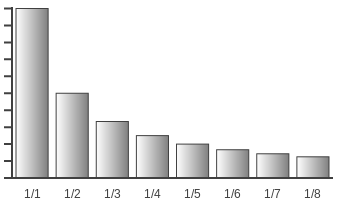
\includegraphics[width=0.7\linewidth]{zipf_graph}
	\caption[A perfect example of what Zipf's law would look like on a graph]{}
	\label{fig:zipfgraph}
\end{figure}

Zipf’s law was formulated using mathematical statistics refering to how many types of data studied in  physical and social sciences, the rank-frequency distribution is an inverse relation. A ranked frequency distribution is the distribution of size by frequency, in decreasing order of usage. An inverse rank frequency distributionis the inverse of frequency in decreasing order. Zipf's law states that given a body of natural words, the frequency of any word is inversely proportional to its rank in the frequency table. It states the most used word in a language is used twice as much as the second most used word, and three times as much as the third, and so on. If the most frequent term occurs x amount of times, the second most frequent term has half as many occurrences, and the third most frequent term has a third as many occurrences, and so on. 

\begin{equation}
  P(x) = \frac{x^{-(\rho+1)}}{\zeta (\rho + 1)'}
\end{equation}

\begin{equation}
  P(x) = \frac{1}{r \ln(1.78 R)'}
\end{equation}


There are a few key components of Zipf’s law that distinguish it from other power laws
What this means in practice is that very few word types account for the vast majority of the word occurrences in a document. 

	

\subsection{Usages}

Zipf's law holds in many areas of study from the popularity of last names, the firing patterns of neural networks, to word frequencies. The most common place Zipf's law is used is in linguistics. Natural language processing uses the empirical law to understand the manner in which people talk, and comprehend knowledge. Individual writing styles can be detected quite accurately by focusing on just these high-frequency, low-semantically valuable words. Those low-semantically valuable words are considered useless in identifying a topic, but can be useful in identifying the author. Every person carries around little behavioral ticks that come across in these little words that are used all the time.  Text compression also takes note of Zipf's law in order to include the most frequently used terms in the compressed text. Recording the repeated words of a text can help people remember what topics are being discussed and what information is important to remember. It takes the idea of an abstract, but allows a computer to do that analysis without human assistance. Although it is frequently used in linguistics, there are other places Zipf's law is found.  
AI powered technology has integrated more and more into daily life. One of the things AI powered machines do is generate text messages. For AI machines to portray the correct message, it must be written in a way that humans can comprehend. Understanding the way humans speak, and their use of repetitive vocabulary provide a better guideline for AI powered text messages. 
The Zipf relationship of inverse frequency ranking occurs in many other rankings of human-created systems, such as the ranks of mathematical expressions, ranks of notes in music, and even in uncontrolled environments. The uncontrolled environments referred to are things such as corporation sizes, income rankings, ranks of the number of people watching the same TV channel, cells' transcriptomes  and so on. The appearance of the distribution in rankings of cities by population was first noticed by Felix Auerbach in 1913, leading to a curiosity of Zipf's law for cities. Zipf's law can be used to calculate the population size of cities. Theoretcially, a researcher would not need the yearly census to determine the population of a city. A researcher would only need to know how Zipf's law works, so they can apply it to human created systems. 
The allocation of resources is also something the government must distribute. If an urban planner, who works for the government, has a basic idea of Zipf's law, they would be able to disrtibute resources equitably. The distribution of resources is a big problem to be solved, but perhaps there's a simpler way to determine those needs. even outside of linguistics, Zipf's law appears to be useful in many other fields. thwere would be no point in studying a theory if it could not be applied in the real world.
	

\section{Methods}

There are many ways to go about finding the frequency distribution of words. However, there are certain steps that must be taken no matter what the code looks like.  

\subsection{Choosing datasets}

The Gutenberg Library is an amazing source for free, open source text. There were two ways I could go about choosing data. I could either get as many texts as I could that would all be in different languages. For this first option, I would have texts in different languages, but they would also not be the same text. Those texts would follow different stories, and provide useless data for comparison. If I were to compare texts to each other, they had to be the same text. My second option would be more focused on comparing different translations of text to each other. This would provide more precise data, which would leave less room for unacounted variables. The books I found with the most translations was the sequel of the Odyssey and the Iliad. The Odyssey and The Iliad are available in English, Spanish, French, Latin, and Greek.These were enough translations to work with, so I settled for Homer's books. 


\subsection{Parsing Text}

Parsing text is the cleaning of text, so it may be further analyzed. Researchers do this in order to remove any extra items that aren’t needed in the dataset they are analyzing. The way text would be parsed was by removing the footer, the header, and punctuation. Each book in the Gutenberg library  has a header and footer that state where the book started and ended. Knowing where the header ended and the footer started was useful, because I needed to know where to cut it out. After the header and footer have been removed, punctuation is next. In this project, punctuation is not being analyzed, so it does no good to thsi particular data set. Once punctuation is removed, I tokenized by words. tokenizing by words would select all words without their strings. Once words have been tokenized, the next step is running the analysis.

\subsection{Finding the Frequency Distribution}

To find the frequency distribution, 

\section{Results}

After analyzing translations of The Odyssey and The Iliad in Latin, English, French, Spanish, and Greek, there have been a few conclusions that can be drawn jsut upon looking at the graphs. The most obvious result to note is that all the graphs look almost identical to one another. Although the texts are from the same book, there is little change cause by language translation. All the graphs follow Zipf's law. Unsuprisingly, the most frequently used words had low semantic value, meaning that those words are articles, and provide no context to the text. The most frequently used words are words that are there mostly for grammar. The most frequently used word from each text was the word, ``the''. This comes as no suprise, because in the English language alone, one in every sixteen words said is, ``the''. Although the result was guaranteed, it is still extrodinary how this arises. The repetition of human langauge is something that will never cease to amaze. The patterns that nature makes are astounding. Now, we must explain why it happens. 


\subsection{Causes}

Although it is known that Zipf's law appears everywhere, it does not answer why it appears everywhere. There is not proven answer as to why it occurs, but there are many theories out there. A discrete for of Pareto's Principle is seen in graphs of Ziph's law. The Pareto Principle states that around 20 percent of the causes are responsible for 80 percent of the outcomes. Just like with Zipf's law, Pareto's Principle of Distribution is seen in many areas, but here are a few examples. In language, the most frequently used 18 percent of words account for 80 percent of all word occurences. The richest 20% of humans have 82.7 percent of the world's income. In the the United Sattes, 20% of pMEDICAL PETIENTS USE 80 PERCENT OF ALL HEALTH CARE RESOURCES. Taking Pareto's law case by case, could help identify why Zipf's law occurs. In addition, there is more research done on Pareto's principle, so with more information

\subsubsection{Principle of Least Effort}

There is one explanation that Zipf himself proposed, and that is the principle of least effort. The principle of least effort is a broad theory which suggests that animals, people, and even well-designed machines will naturally choose the path of least resistance or "effort". In the late 1940’s, Zipf studied this law. In that decade he published a book titled, “Human Behaviour and the Principle of Least Effort: An Introduction to Human Ecology”. He proposed that neither speakers nor hearers using a given language want to work any harder than necessary to reach understanding, and the process that results in approximately equal distribution of effort leads to the observed. He theorized that the distribution of word use was due to tendency to communicate efficiently with least effort, also known as Zipf’s law. 


\subsubsection{Probability of Chance}

Some researches argue that for language, the explanation is even simpler than imagined. A few years after Zipf published his paper, Menort Mandelbert showed that there may be nothing mysterious about Zipf's law at all. If a person, or even in his experiment, a monkey, randomly typed on a keyboard, they will produce words distributed according to Zipf's law. The reason this happens is because there are exponentially more different long words than short words. If all 26 letters on a keyboard, including the space bar are equally likely to be typed, after a letter has been typed and a word has begun, the probability that the next input being typed is the space bar, is one in twenty seven.  If someone randomly generates  characters, about one in every 27 or 3.7 percent of the input between spaces, will be a single letter. Our mysterious distribution has been created out f nothing but the inevitabilities of math. Is language just as random as typing character in a keyboard.


\subsection{Critical Points}

Critical points may also play a role in the causation of Zipf's law. In writing and in conversation, speakers tend to stick to a topic. Even if, say in conversation, a person meanders off topic, there is still some type of segway that leads them in to teh following thought. Speakers and writers have a reason to speak, and that's because they're saying something. Humans do not randomly choose words randomly. There is a union between their words. Conversations and literature aren't random. They have a purpose, so when a discussion is being had, they tend to repeat their point many times. The same vocabulary may show up repetitively, because that is what they are discussing. In literature, as well as in natural language, the topic of discussion is stuck with until a critical point is read. The critical point in a conversation is the moment when an agreement, conclusion, or turning point happens. Once the critical point of a conversation is reached, the subject is changed, and the vocabulary shifts. This is the way language flows. A topic is discussed, vocabulary specific to that topic is used, a critical point is met, and the subject changes. The critical point theory applies in small portions of text, but cannot apply in larger texts. Critcial points can be seen in short discussions, where the subject does not change, for at least a couple minutes. Paragraphs would also be a place where critical point theory could be used, because only one topic is discussed. However, once we look in to books, or even a chapter in a book, there is so much topic change that the main vocabulary for each topic does not stand out. 

\subsubsection{Preferential Attachment}

Although randomness can explain a monkey recieveing Zipf's distribution of text, that's not the way humans communicate. Language is deterministic, and carefully chosen. People don't just select unrelated words to follow after the next. What follows a sentence is the result of what was stated in the sentence before. Perhaps there is a way that thoughts and topics of discussion ebb and flow that contribute to Zipf's law. Maybe distributions occur through processes that chart change according to how they've previously operated. These are called preferential attachment processes. They occur when something is given out according to how much is already possessed. The more views a post gets, the more likely it is to be recommended to other individuals, which will attract even more views. Take a rolling snowball for example, the more the snowball rolls, the more snow it accumulates, expanding its surface area to collect more snow. The more snow that accumulates, the larger the surface area extends, the more snow a snowball can accumulated. Essentially, the big get bigger. There does not have to be a deliberate choice driving preferential attachment. It can happen naturally. This is seen in everyday life. Another note-able example, "The rich get richer", derives from preferential attachment processes. It's just math. Perhaps Zipf's law is, if not caused by, but at least strengthened by preferential attachment. Once a word is used, it is more likely to be used again.

	

\section{Discussion}

\subsection{Importance}

Zipf’s law articulates how much recycling of language people do. It is a question that further looks into human vocabulary, and leads to other philosophical questions. Why do people use the same words over and over again when there are hundreds of thousands to choose from in the English language alone? What’s more, is this law of distribution works nearly the same in all languages. What is the importance of certain filler words such as, “ the, and, of, it…” These essentially useless articles are what make up a large portion of human vocabulary. Why is the word, "the" given so much meaning?


\subsection{Problems with Zipf's Law}

When looking at a table distribution of Zipf’s la the most frequently used words fall on the left side, and because words on the left side of your graph occur very frequently and words on the right very infrequently. The most frequently used terms carry a lot more information from a mathematical point of view. However, it carries a lot less information from a semantic point of view. “The,” “and,” and “of,” are not the most interesting words. If your question is about what makes documents different at the level of content or theme, then these words won’t tell you what you want to know. If one is analyzing text using Zipf’s law to extract the theme of the paper, they will go no where. 
• Zipf's law for words suffers from three main problems: its formulation is ambiguous, its validity has not been tested rigorously from a statistical point of view, and it has not been confronted to a representatively large number of texts.
• Makes most frequent errors for highest frequency and lowest frequency words 
• It has been analyzed in more than 30,000 English texts. The goodness of fit tests yield that only about 15% of the texts are statistically compatible with this form of Zipf's law.


\section{Conclusions}


\subsection{Why Zipf's Law Ocurrs}

Things are distributed in a myriad of ways, not just power laws. Language is personal and intentional, so why does all language end up following a predetermined cycle. What about the world and humans could cause such complex activities and behaviors to follw such a simple rule? The answer is still undetermined, but there are a number of theories that, when joined together, explain Zipf's law.  


\section*{Acknowledgments}

The most gracious thanks to Mark Galassi must be given. He worked with me for hours and taught me how to code. This would not be possible without him, and his willingness to put up with me. Rachel Hopkins was assigned to be my mentor for this project. She pushed brilliant ideas on me, and nudged me into the right direction. Thank you Rachel! The past four weeks have been spent in the most beautiful office thanks to Optiver. Their team has so much insight on everything STEM. They have treated us to the most lush, and cushy work environment. It's gonna be hard to adjust to normal life after being fed oreos everyday. This oppurtunity would not be possible without Optiver. Thank you for hosting us at your Austin office. Finally, I would like to thank the Institute for Computing in Research for thsi amazing oportunity. It has been an academically chanllenging 4 weeks, but I've learned things I couldn;t have learned in a classroom. Thank you to evveryone who has helped these past couple weeks. It's been an honor working with y'all.
During my internship with the Institute for Computing in Research, Optiver 

%%% ----- BIBLIOGRAPHY -----

\bibliographystyle{apalike} 
\bibliography{BIBLIO_Zipf} 



\end{document}
